% L13a figure: JSON text and the tree of data that it describes.
%
% Left: part of the body of the National Weather Service points response for
% Ithaca, NY. Right: the same data as a tree. Blue outlines mark the containers
% (objects and an array), gray boxes mark the values, and each line carries the
% key of the value that it leads to.
%
% Drawn on November 12, 2026 with the palette and build of the L12c figures.
% The notebook SVG carries a dark palette added by theme_svg.py; keep new colors
% in that script's mapping when changing the palette here.
\documentclass[tikz,border=4pt]{standalone}
\usepackage[no-math]{fontspec}
\IfFontExistsTF{Arial}{\setsansfont{Arial}}{\setsansfont{TeX Gyre Heros}}
\IfFontExistsTF{Menlo}{\setmonofont{Menlo}[Scale=0.88]}{}
\renewcommand{\familydefault}{\sfdefault}
\usepackage{amsmath,amssymb}
\usetikzlibrary{arrows.meta, calc, fit, backgrounds, positioning, decorations.pathreplacing}

% Ink, blue, gray, and band match the L12c figures.
\definecolor{vnink}{HTML}{202124}
\definecolor{gdblue}{HTML}{0091FF}
\definecolor{gdgray}{HTML}{6D7278}
\definecolor{waband}{HTML}{EEF0F2}
\definecolor{nodefill}{HTML}{FFFFFF}

\begin{document}
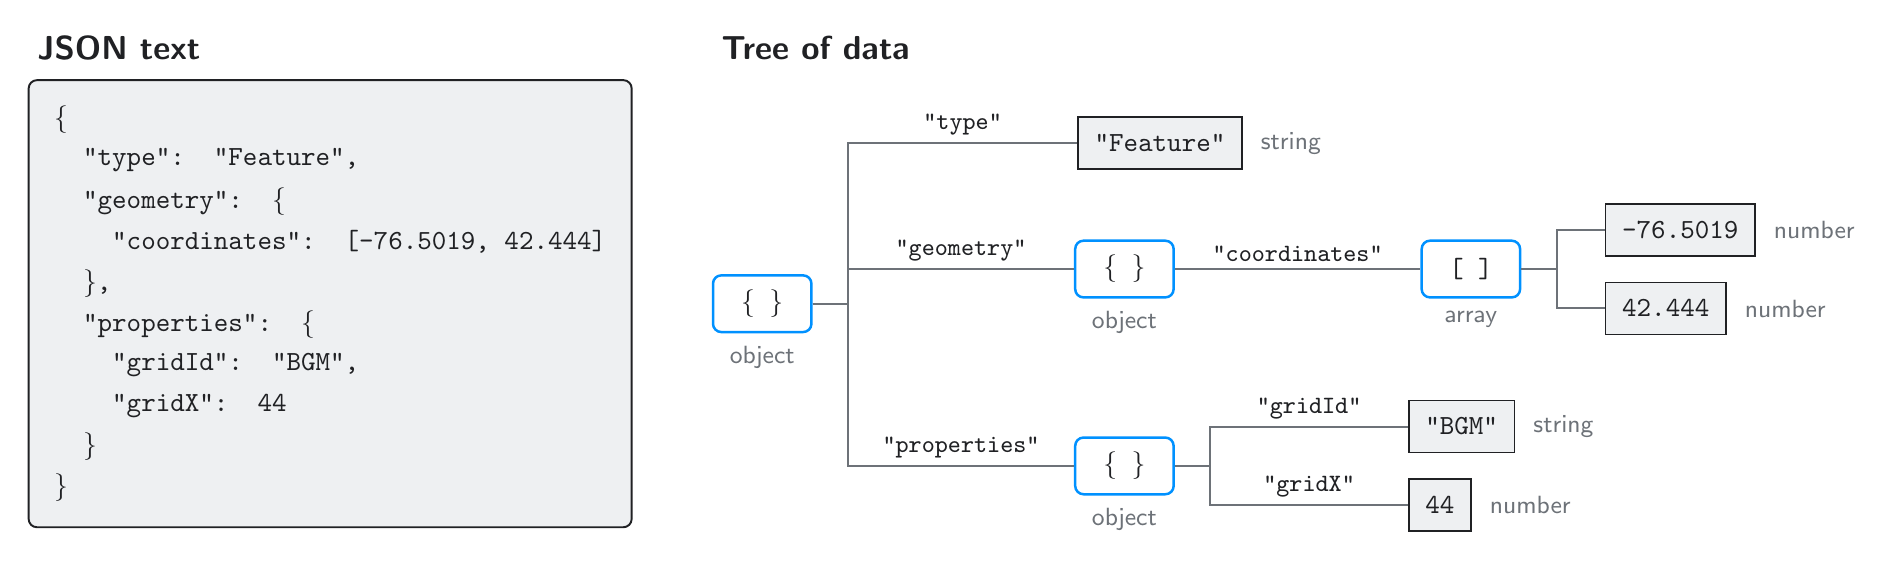
\begin{tikzpicture}[
  font=\sffamily\large,
  ln/.style={anchor=west, font=\ttfamily\normalsize, text=vnink, inner sep=0pt},
  panel/.style={draw=vnink, rounded corners=3pt, fill=waband, line width=0.7pt, inner sep=9pt},
  title/.style={font=\sffamily\large\bfseries, text=vnink, anchor=south west},
  box/.style={draw=gdblue, rounded corners=3pt, fill=nodefill, line width=0.9pt, font=\ttfamily\normalsize,
    text=vnink, minimum width=1.25cm, minimum height=0.72cm, inner sep=3pt},
  leaf/.style={draw=vnink, fill=waband, line width=0.6pt, font=\ttfamily\normalsize, text=vnink,
    minimum height=0.66cm, inner xsep=6pt, inner ysep=3pt, anchor=west},
  kind/.style={font=\sffamily\small, text=gdgray},
  key/.style={font=\ttfamily\small, text=vnink, inner sep=2.5pt},
  edge/.style={draw=gdgray, line width=0.7pt}
]

% ------------------------------------------------------------------ the JSON text
\node[ln] (t1)  at (0, 0.00) {\{};
\node[ln] (t2)  at (0,-0.52) {\ \ "type": "Feature",};
\node[ln] (t3)  at (0,-1.04) {\ \ "geometry": \{};
\node[ln] (t4)  at (0,-1.56) {\ \ \ \ "coordinates": [-76.5019, 42.444]};
\node[ln] (t5)  at (0,-2.08) {\ \ \},};
\node[ln] (t6)  at (0,-2.60) {\ \ "properties": \{};
\node[ln] (t7)  at (0,-3.12) {\ \ \ \ "gridId": "BGM",};
\node[ln] (t8)  at (0,-3.64) {\ \ \ \ "gridX": 44};
\node[ln] (t9)  at (0,-4.16) {\ \ \}};
\node[ln] (t10) at (0,-4.68) {\}};
\begin{scope}[on background layer]
  \node[panel, fit=(t1)(t2)(t3)(t4)(t5)(t6)(t7)(t8)(t9)(t10)] (txt) {};
\end{scope}
\node[title] at ($(txt.north west)+(0,0.12)$) {JSON text};

% ------------------------------------------------------------------ the tree
\node[box] (root) at (9.0,-2.34) {\{ \}};
\node[kind, below=1pt of root] {object};

\node[leaf] (type) at (13.0,-0.30) {"Feature"};
\node[kind, right=3pt of type] {string};

\node[box] (geo) at (13.6,-1.90) {\{ \}};
\node[kind, below=1pt of geo] {object};
\node[box] (coords) at (18.0,-1.90) {[ ]};
\node[kind, below=1pt of coords] {array};
\node[leaf] (lon) at (19.7,-1.40) {-76.5019};
\node[kind, right=3pt of lon] {number};
\node[leaf] (lat) at (19.7,-2.40) {42.444};
\node[kind, right=3pt of lat] {number};

\node[box] (prop) at (13.6,-4.40) {\{ \}};
\node[kind, below=1pt of prop] {object};
\node[leaf] (gid) at (17.2,-3.90) {"BGM"};
\node[kind, right=3pt of gid] {string};
\node[leaf] (gx) at (17.2,-4.90) {44};
\node[kind, right=3pt of gx] {number};

\node[title] at ($(root.west |- txt.north)+(0,0.12)$) {Tree of data};

% each line carries the key of the value that it leads to
\draw[edge] (root.east) -- ++(0.45,0) |- (type.west) node[key, pos=0.75, above] {"type"};
\draw[edge] (root.east) -- ++(0.45,0) |- (geo.west) node[key, pos=0.75, above] {"geometry"};
\draw[edge] (root.east) -- ++(0.45,0) |- (prop.west) node[key, pos=0.75, above] {"properties"};
\draw[edge] (geo.east) -- (coords.west) node[key, midway, above] {"coordinates"};
\draw[edge] (coords.east) -- ++(0.45,0) |- (lon.west);
\draw[edge] (coords.east) -- ++(0.45,0) |- (lat.west);
\draw[edge] (prop.east) -- ++(0.45,0) |- (gid.west) node[key, pos=0.75, above] {"gridId"};
\draw[edge] (prop.east) -- ++(0.45,0) |- (gx.west) node[key, pos=0.75, above] {"gridX"};

\end{tikzpicture}
\end{document}
